\documentclass[conference]{IEEEtran}
\IEEEoverridecommandlockouts
% The preceding line is only needed to identify funding in the first footnote. If that is unneeded, please comment it out.
\usepackage{cite}
\usepackage{hyperref}
\usepackage{amsmath,amssymb,amsfonts}
\usepackage{graphicx}
\usepackage{textcomp}
\usepackage{xcolor}
\usepackage{pgfplots}
\pgfplotsset{compat=1.18}
\usepackage{tikz}
\usepackage{subcaption}
\usepackage{booktabs}
\usetikzlibrary{shapes,arrows,positioning,fit,calc}

\def\BibTeX{{\rm B\kern-.05em{\sc i\kern-.025em b}\kern-.08em
    T\kern-.1667em\lower.7ex\hbox{E}\kern-.125emX}}

\begin{document}

\title{DTS: Delta-Based Tile Scoring for Accelerating Long-Context Attention\\}

\author{\IEEEauthorblockN{Anonymous Authors}
\IEEEauthorblockA{\textit{Affiliation} \\
\textit{Organization}\\
City, Country \\
email@domain.com}
}

\maketitle

\begin{abstract}
Long-context inference in large language models is constrained by the quadratic computational complexity of self-attention. To address this, we leverage the high sequential similarity of adjacent query and key vectors to propose Delta-based tile scoring (DTS). DTS uses content-adaptive subsets of these vectors to efficiently estimate tile importance for block-sparse attention. Experiments on LLaMA-3.1-8B-Instruct demonstrate that DTS closely matches full attention accuracy on RULER and LongBench while achieving a 3.3× end-to-end prefill speedup at a 512K context length. Furthermore, DTS generalizes across architectures and modalities. Importantly, it achieves these results while maintaining a substantially lower scoring cost than XAttention.

\end{abstract}

\begin{IEEEkeywords}
sparse attention, LLM inference, long context, hardware acceleration
\end{IEEEkeywords}

\section{Introduction}




Long-context inference has become a critical and impactful application for Large Language Models (LLMs)~\cite{dubey2024llama3, qwen25, Qwen2-VL, reid2024gemini, liu2023ring}. For instance, coding agents~\cite{yang2024sweagent} ingest entire codebases to reason about them, while other systems analyze extensive documents such as legal contracts, research papers, and financial reports. Furthermore, Retrieval-Augmented Generation (RAG)~\cite{lewis2020retrieval} integrates retrieved documents directly into the model context, grounding LLM responses in external knowledge. However, all these applications share a common bottleneck.


LLM inference consists of two stages: the prefill stage, which processes the entire input prompt in a single forward pass, and the decoding stage, which generates output tokens one by one. During the prefill stage, computing self-attention performs a computation that is quadratic in complexity, as each token must communicate with every other token.
\begin{figure}[t]
    \centering
    \input{diagrams/dts_3part.tex}
    \caption{DTS four-stage process: Compress queries and keys into $\hat{Q}$ and $\hat{K}$ and multiply them to estimate sparse attention scores during delta scoring. These individual scores are then summed to yield a single importance score for each tile. Finally, the highest-scoring tiles are selected to undergo block sparse attention.}
    \label{fig:dts_flow}
\end{figure}

As context length grows, the quadratic complexity of attention makes prefill increasingly expensive.
Memory was the original wall; FlashAttention~\cite{dao2022flashattention, dao2023flashattention2, shah2024flashattention3} and PagedAttention~\cite{kwon2023efficient} removed it but did not address the time complexity: computing attention on long contexts is slow.

A large body of work aims to accelerate attention for long context tasks by exploiting the empirical sparsity of the attention matrix: most tokens only attend strongly to a small local window and a few distant positions, so many token pair interactions do not need to be computed at all.
Early work used fixed sparse patterns~\cite{child2019generating, Beltagy2020Longformer, zaheer2020bigbird}; more recent methods determine the pattern dynamically based on the input~\cite{jiang2024minference, lai2025flexprefill, xu2025xattention}.

This paper exploits the insight that adjacent tokens have similar key vectors, with high cosine similarity between neighboring keys. This redundancy in $K$ is already documented in prior work~\cite{wang2024kvmerger, qi2024deltallm}. We show that the same holds for query vectors: adjacent queries are also highly similar. 

We apply this insight as a tile importance estimator for block-sparse attention, choosing which tiles to compute while sampling far less of each tile than existing estimators.

\section{Related Work}

The dominant strategy in attention acceleration is exploiting the fact that attention matrices are empirically sparse: most tokens attend strongly to only a small fraction of others.
Child et al.~\cite{child2019generating}, along with subsequent works like Longformer~\cite{Beltagy2020Longformer} and BigBird~\cite{zaheer2020bigbird}, were among the first to demonstrate this, observing that trained Transformer attention matrices concentrate on local windows and a few distant positions.
They proposed fixed sparse patterns (local windows combined with strided or fixed summary positions) to approximate full attention with fewer FLOPs.
The limitation is that a fixed pattern cannot adapt to the content of a given input. This motivated a shift to dynamic sparse attention, where the sparsity pattern is determined on the fly. These methods generally fall into two categories: attention shape methods and block-sparse attention methods.

\textbf{Block-sparse attention methods} dynamically skip attention tiles that are estimated to be unimportant. SpargeAttn~\cite{zhang2025spargeattn} selects a representative per block using mean pooling and scores tiles based on the block representatives. XAttention~\cite{xu2025xattention} uses the sum of antidiagonal values within each attention block as a lightweight proxy for tile importance. Both methods then compute attention only for the tiles scored as important.

\textbf{Attention shape methods}, in contrast, identify and exploit the specific attention pattern a head exhibits. For example, MInference~\cite{jiang2024minference}---a foundational and widely deployed approach---observes that LLM attention heads follow consistent structural patterns (A-shape, Vertical-Slash, and Block-Sparse) across inputs. It assigns each head its dominant pattern offline and builds sparse indices accordingly at inference time. Crucially, Block-Sparse heads lack a fixed, exploitable shape; for these, MInference falls back to block-sparse attention. Similar to SpargeAttn, it mean-pools each query and key block into a single representative and uses the resulting attention scores to select important tiles.

FlexPrefill~\cite{lai2025flexprefill} extends MInference by making it content-adaptive. Instead of assigning a shape to a head offline, FlexPrefill decides at inference time whether to treat a head as Vertical-Slash or block-sparse, based on the Jensen-Shannon divergence between the head's attention and each candidate pattern. It also differs in how tiles are selected.



Our Delta-based tile scoring (DTS) is most closely related to XAttention~\cite{xu2025xattention} and SpargeAttn~\cite{zhang2025spargeattn}. All three methods compute a cheap importance score to identify which tiles require exact computation. While XAttention sums the antidiagonal values of each block and SpargeAttn mean-pools blocks into single representatives, DTS compresses $Q$ and $K$ to perform a lightweight attention that captures tile importance. Furthermore, unlike XAttention's reliance on rigid strides, DTS's tile scoring remains fully content-adaptive.

\section{Observations}
\label{sec:observations}

High cosine similarity between adjacent key states has been previously observed~\cite{wang2024kvmerger}.

In this section, we extend this analysis to both key and query states. We feed LLaMA-3.1 8B Instruct a sequence of 512 tokens sampled from WikiText-103 and record the states at layers 0, 8, 16, and 23. At each layer, we compute the average cosine similarity between all adjacent token pairs, averaged over heads.
We compare two configurations: (1) \textbf{Natural Order (post-RoPE)}: states computed with the original token sequence, and (2) \textbf{Shuffled Order}: states computed after randomly shuffling the token positions, breaking positional adjacency.

Comparing the shuffled and natural orders allows us to isolate the source of the similarity. As shown in Figure~\ref{fig:combined_similarity}, both key and query states exhibit high adjacent cosine similarity in their natural order. When the token order is shuffled, the similarity drops significantly for both keys and queries. This confirms that the high adjacent similarity is not solely an artifact of the projection matrices or positional encodings, but is strongly driven by the inherent semantic and structural redundancy of adjacent tokens in natural text.
Crucially, query states exhibit the same high local redundancy as key states, motivating a compression strategy that exploits both.

\begin{figure}[!ht]
\centering
\resizebox{\linewidth}{!}{
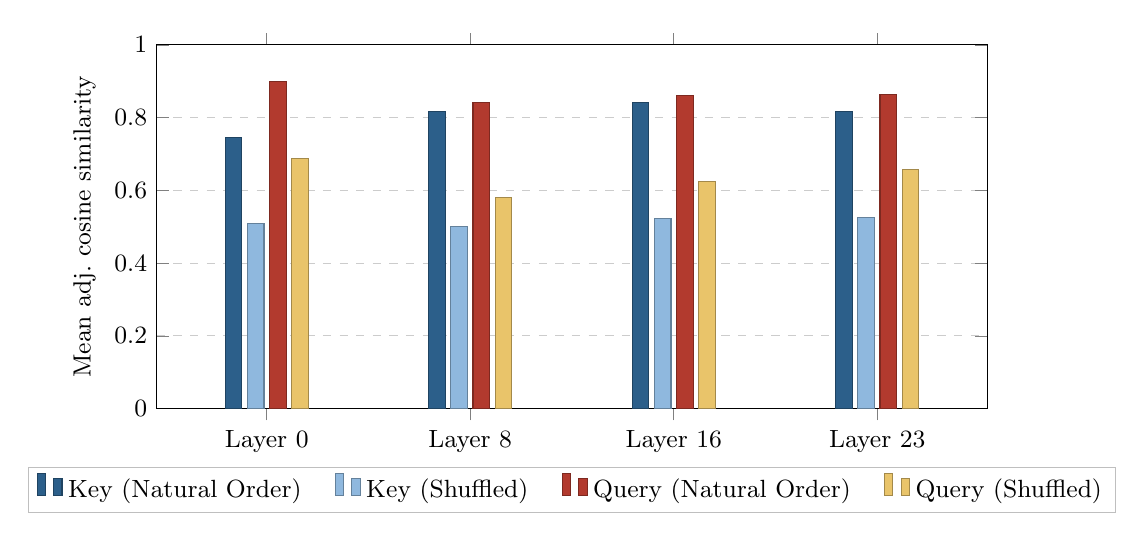
\begin{tikzpicture}
  \definecolor{keyReal}{HTML}{2C5F8A}   % dark blue
  \definecolor{keyShuf}{HTML}{8FB8DE}   % light blue
  \definecolor{queryReal}{HTML}{B23A2E} % dark red
  \definecolor{queryShuf}{HTML}{E9C46A} % light amber
  \begin{axis}[
    ybar,
    bar width=6pt,
    width=\textwidth,
    height=6.2cm,
    enlarge x limits=0.18,
    ymin=0, ymax=1,
    ytick={0,0.2,0.4,0.6,0.8,1.0},
    ylabel={Mean adj.\ cosine similarity},
    symbolic x coords={Layer 0, Layer 8, Layer 16, Layer 23},
    xtick=data,
    tick label style={font=\small},
    ylabel style={font=\small},
    ymajorgrids=true,
    grid style={dashed, gray!40},
    legend style={
      at={(0.5,-0.16)}, anchor=north,
      legend columns=4, font=\small,
      /tikz/every even column/.append style={column sep=10pt},
      draw=gray!50,
    },
  ]
    \addplot[fill=keyReal,   draw=keyReal!70!black]   coordinates {(Layer 0,0.7457) (Layer 8,0.8167) (Layer 16,0.8423) (Layer 23,0.8172)};
    \addplot[fill=keyShuf,   draw=keyShuf!70!black]   coordinates {(Layer 0,0.5094) (Layer 8,0.5005) (Layer 16,0.5216) (Layer 23,0.5242)};
    \addplot[fill=queryReal, draw=queryReal!70!black] coordinates {(Layer 0,0.9000) (Layer 8,0.8408) (Layer 16,0.8619) (Layer 23,0.8626)};
    \addplot[fill=queryShuf, draw=queryShuf!70!black] coordinates {(Layer 0,0.6880) (Layer 8,0.5807) (Layer 16,0.6234) (Layer 23,0.6570)};
    \legend{Key (Natural Order), Key (Shuffled), Query (Natural Order), Query (Shuffled)}
  \end{axis}
\end{tikzpicture}
}
\caption{Average cosine similarity of adjacent key and query states for LLaMA-3.1 8B Instruct, showing both natural token order (post-RoPE) and randomly shuffled token order.}
\label{fig:combined_similarity}
\end{figure}


\section{Methodology}

In this section, we describe the core components of our proposed approach: Delta Packing and its extension to Delta-Based Tile Scoring (DTS). 

\subsection{Delta Packing}
The foundational operation in our methodology is Delta Packing. Adjacent query and key vectors are highly similar at the token level, which means they can be compressed along the sequence dimension. 

Algorithm 1 outlines the sequential Delta Packing procedure.

\begin{figure}[htbp]
\noindent\hrulefill\\
\textbf{Algorithm 1: Sequential Delta Packing}\\[-2mm]
\noindent\hrulefill
\begin{tabbing}
\textbf{Input:} Matrix $\mathbf{K} \in \mathbb{R}^{N \times D}$, similarity threshold $\tau$ \\
\textbf{Output:} Packed matrix $\hat{\mathbf{K}}$, binary mask $\Delta \in \{0, 1\}^N$ \\
1. \quad \= $\Delta \gets \mathbf{0}$, $\Delta[0] \gets 1$ \\
2. \> $\mathbf{k}_{\text{anchor}} \gets \mathbf{K}[0]$ \\
3. \> \textbf{for} $i = 1$ \textbf{to} $N-1$ \textbf{do} \\
4. \> \quad \= \textbf{if} $\cos(\mathbf{K}[i], \mathbf{k}_{\text{anchor}}) < \tau$ \textbf{then} \\
5. \> \> \quad \= $\Delta[i] \gets 1$ \\
6. \> \> \> $\mathbf{k}_{\text{anchor}} \gets \mathbf{K}[i]$ \\
7. \> \> \textbf{end if} \\
8. \> \textbf{end for} \\
9. \> $\hat{\mathbf{K}} \gets \mathbf{K}[\Delta == 1]$ \\
10.\> \textbf{return} $\hat{\mathbf{K}}, \Delta$
\end{tabbing}
\vspace{-4mm}
\noindent\hrulefill
\end{figure}

\textbf{Parallel Delta Packing.}
In practice, we apply sequential delta packing to fixed-size chunks (e.g., 128 tokens) independently by setting each chunk's first vector as an anchor, which breaks the sequential dependency. Otherwise, sequential packing has a linear time complexity with respect to sequence length, which would result in severe overhead in extremely long contexts.



\subsection{Delta-Based Tile Scoring (DTS)}
Building upon the Delta Packing concept, we introduce Delta-Based Tile Scoring (DTS) for block-sparse attention. 

The DTS methodology operates as follows:
\begin{enumerate}
    \item \textbf{Delta Pack:} Apply Delta packing on \textbf{Q} and \textbf{K} separately.
    \item \textbf{Multiply:} Multiply the packed $\hat{\textbf{Q}}$ and $\hat{\textbf{K}}$ to get representative attention scores in tiles.
    \item \textbf{Sum:} Sum the tile attention scores to get an importance score for each tile.
    \item \textbf{Normalize:} Apply softmax to the tile scores across query rows to obtain tile weights.
    \item \textbf{Threshold:} Select the highest-scoring tiles per row until their accumulated weights exceed a threshold $\tau = 0.9$.
    \item \textbf{Compute:} Process the selected tiles using block-sparse attention and skip the remaining tiles.
\end{enumerate}



Figure~\ref{fig:delta_tile_scoring} provides a detailed algorithmic view of how \textbf{Q} and \textbf{K} are packed into $\hat{\textbf{Q}}$ and $\hat{\textbf{K}}$, and how these packed matrices are multiplied to obtain the sparse attention scores.

Figure~\ref{fig:dts_flow} illustrates the complete end-to-end flow of this four-stage methodology, showcasing how the sparse attention scores are summed to compute tile importance, and how these tile scores determine which tiles are processed and which are skipped.

\begin{figure}[!ht]
\centering
\resizebox{\columnwidth}{!}{
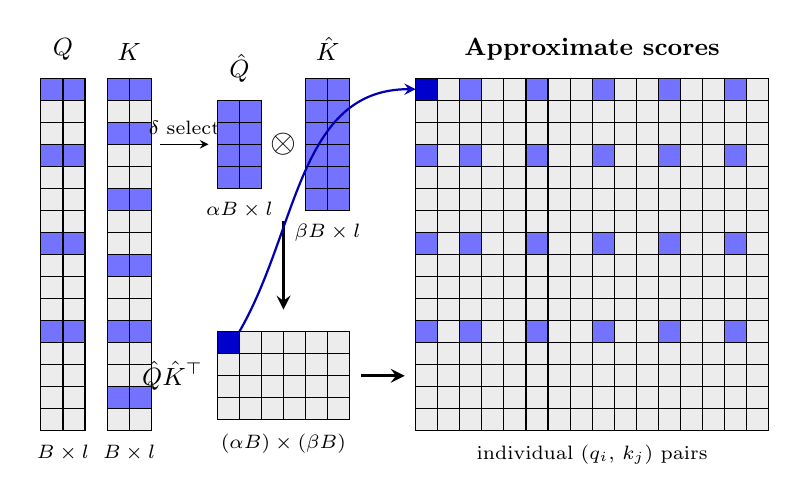
\begin{tikzpicture}
  \def\cell{0.28}
  \colorlet{hilightA}{blue!55}
  \colorlet{hilightFocus}{blue!80!black}
  \colorlet{plain}{gray!15}

  % Q anchors: rows 0, 3, 7, 11   (4 of 16)
  % K anchors: rows 0, 2, 5, 8, 11, 14  (6 of 16)

  %--- Full Q (16 rows × 2 cols) ---
  \foreach \r in {0,...,15} {
    \pgfmathtruncatemacro{\isanchor}{
      (((\r==0)+(\r==3)+(\r==7)+(\r==11))>0) ? 1 : 0
    }
    \foreach \c in {0,1} {
      \ifnum\isanchor=1 \fill[hilightA] \else \fill[plain] \fi
        ({\c*\cell},{-\r*\cell}) rectangle ({(\c+1)*\cell},{(-\r-1)*\cell});
      \draw ({\c*\cell},{-\r*\cell}) rectangle ({(\c+1)*\cell},{(-\r-1)*\cell});
    }
  }
  \node[above, font=\small\bfseries] at ({1*\cell}, 0.1)             {$Q$};
  \node[below, font=\scriptsize]     at ({1*\cell},{-16*\cell-0.05}) {$B \times l$};

  %--- Full K (16 rows × 2 cols) ---
  \foreach \r in {0,...,15} {
    \pgfmathtruncatemacro{\isanchor}{
      (((\r==0)+(\r==2)+(\r==5)+(\r==8)+(\r==11)+(\r==14))>0) ? 1 : 0
    }
    \foreach \c in {0,1} {
      \ifnum\isanchor=1 \fill[hilightA] \else \fill[plain] \fi
        ({(3+\c)*\cell},{-\r*\cell}) rectangle ({(4+\c)*\cell},{(-\r-1)*\cell});
      \draw ({(3+\c)*\cell},{-\r*\cell}) rectangle ({(4+\c)*\cell},{(-\r-1)*\cell});
    }
  }
  \node[above, font=\small\bfseries] at ({4*\cell}, 0.1)             {$K$};
  \node[below, font=\scriptsize]     at ({4*\cell},{-16*\cell-0.05}) {$B \times l$};

  %--- Delta-select arrow ---
  \draw[-{stealth}] ({5.4*\cell},{-3*\cell}) -- ({7.6*\cell},{-3*\cell});
  \node[above, font=\scriptsize] at ({6.5*\cell},{-3*\cell}) {$\delta$ select};

  %--- \hat{Q} (4 rows × 2 cols) ---
  \foreach \r in {0,...,3} {
    \foreach \c in {0,1} {
      \fill[hilightA]
        ({(8+\c)*\cell},{-(1+\r)*\cell}) rectangle ({(9+\c)*\cell},{-(2+\r)*\cell});
      \draw ({(8+\c)*\cell},{-(1+\r)*\cell}) rectangle ({(9+\c)*\cell},{-(2+\r)*\cell});
    }
  }
  \node[above, font=\small\bfseries] at ({9*\cell},{-1*\cell+0.1})       {$\hat{Q}$};
  \node[below, font=\scriptsize]     at ({9*\cell},{-5*\cell-0.05}) {$\alpha B \times l$};

  %--- ⊗ ---
  \node[font=\large] at ({11*\cell},{-3*\cell}) {$\otimes$};

  %--- \hat{K} (6 rows × 2 cols) ---
  \foreach \r in {0,...,5} {
    \foreach \c in {0,1} {
      \fill[hilightA]
        ({(12+\c)*\cell},{-\r*\cell}) rectangle ({(13+\c)*\cell},{-(1+\r)*\cell});
      \draw ({(12+\c)*\cell},{-\r*\cell}) rectangle ({(13+\c)*\cell},{-(1+\r)*\cell});
    }
  }
  \node[above, font=\small\bfseries] at ({13*\cell}, 0.1)       {$\hat{K}$};
  \node[below, font=\scriptsize]     at ({13*\cell},{-6*\cell-0.05}) {$\beta B \times l$};

  %--- Downward Flow Arrow ---
  \draw[-{stealth}, very thick] ({11*\cell},{-6.5*\cell}) -- ({11*\cell},{-10.5*\cell});

  %--- (αB)×(βB) result matrix: 4 rows × 6 cols ---
  \foreach \r in {0,...,3} {
    \foreach \c in {0,...,5} {
      \pgfmathtruncatemacro{\isFocus}{(\r==0)*(\c==0)}
      \ifnum\isFocus=1
        \fill[hilightFocus]
      \else
        \fill[plain]
      \fi
        ({(8+\c)*\cell},{-(11.5+\r)*\cell}) rectangle ({(9+\c)*\cell},{-(12.5+\r)*\cell});
      \draw ({(8+\c)*\cell},{-(11.5+\r)*\cell}) rectangle ({(9+\c)*\cell},{-(12.5+\r)*\cell});
    }
  }
  \node[left, font=\small\bfseries]  at ({7.8*\cell},{-13.5*\cell})    {$\hat{Q}\hat{K}^\top$};
  \node[below, font=\scriptsize]     at ({11*\cell},{-15.5*\cell-0.05}) {$(\alpha B)\times(\beta B)$};

  %--- Rightward Flow Arrow ---
  \draw[-{stealth}, very thick] ({14.5*\cell},{-13.5*\cell}) -- ({16.5*\cell},{-13.5*\cell});

  %--- 16×16 full score matrix ---
  \foreach \r in {0,...,15} {
    \foreach \c in {0,...,15} {
      \pgfmathtruncatemacro{\isHL}{
        (((\r==0)+(\r==3)+(\r==7)+(\r==11))>0) *
        (((\c==0)+(\c==2)+(\c==5)+(\c==8)+(\c==11)+(\c==14))>0)
      }
      \pgfmathtruncatemacro{\isFocus}{(\r==0)*(\c==0)}
      \ifnum\isFocus=1
        \fill[hilightFocus]
      \else
        \ifnum\isHL=1
          \fill[hilightA]
        \else
          \fill[plain]
        \fi
      \fi
        ({(17+\c)*\cell},{-\r*\cell}) rectangle ({(18+\c)*\cell},{-(1+\r)*\cell});
      \draw ({(17+\c)*\cell},{-\r*\cell}) rectangle ({(18+\c)*\cell},{-(1+\r)*\cell});
    }
  }
  \node[above, font=\small\bfseries] at ({25*\cell}, 0.1) {Approximate scores};
  \node[below, font=\scriptsize]     at ({25*\cell}, {-16*\cell-0.05}) {individual $(q_i,\,k_j)$ pairs};

  %--- Arrow from result cell (0,0) to B×B position (0,0) ---
  \draw[-{stealth}, thick, blue!70!black]
      ({9*\cell},{-11.5*\cell})
      to[out=60, in=180]
      ({17*\cell},{-0.5*\cell});

\end{tikzpicture}
}
\caption{Delta-based tile scoring. Delta pre-processing selects content-adaptive anchors (blue) from $Q$ and $K$ independently, producing $\hat{Q}$ and $\hat{K}$. Their product gives an $(\alpha B)\times(\beta B)$ score matrix; each entry (highlighted cell, arrow) corresponds to a single dot product at one position in the full $B\times B$ score tile.}
\label{fig:delta_tile_scoring}
\end{figure}


\subsection{Per-Head $\tau$ Calibration}
A global threshold of $\tau=0.9$ does not strictly guarantee retaining $90\%$ of the true attention mass, because the tile scores are only estimates. To accurately achieve the target retention rate, similar to X-Attention, we perform an offline calibration step. During this step, the threshold $\tau$ is independently tuned for each attention head so that every head reliably retains its target mass. Detailed procedures for this calibration are presented in Appendix~\ref{app:calibration}.

\section{Experimental Setup}

\subsection{Benchmarks}

We evaluate our method on two text benchmarks and one video benchmark. The text benchmarks are evaluated using LLaMA-3.1~\cite{dubey2024llama3} and Qwen2.5~\cite{qwen25}, while the video benchmark uses Qwen2-VL~\cite{Qwen2-VL}.

\subsubsection{Text Benchmarks}

\paragraph{RULER}
RULER is a synthetic, retrieval-heavy benchmark that evaluates models across context lengths typically ranging from 4K to 128K tokens. The standard RULER setup includes 13 tasks with 100 samples per pass, making it computationally expensive. For development and ablations, we employ a lighter setup comprising 30 samples per task across 9 tasks

\paragraph{LongBench}
LongBench is a real-world benchmark featuring tasks such as coding, question answering, and summarization, with context lengths ranging from roughly 3K to 24K tokens. It covers 21 datasets across six task categories: single-document QA, multi-document QA, summarization, few-shot learning, synthetic retrieval, and code completion. We sample 100 instances per task and evaluate our main DTS results on 16 of these tasks.

\subsubsection{Video Benchmarks}

\paragraph{Video-MME}
Video-MME is a long-video understanding benchmark that tests multiple-choice question answering over videos, sampling each video at 1 frame per second. The benchmark comprises 2,700 videos with durations ranging from short (under 2 minutes) to long (30 to 60 minutes). Our main results evaluate the full 2,700-video test set, while our packing threshold ablations use a reduced 200-video subset.

\subsection{Speedup Experiment}

To measure raw attention speedup, we run an isolated prefill test independent of any downstream task, following the latency evaluation in MInference~\cite{jiang2024minference}. The model is fed a randomly sampled sequence from WikiText-103 across a range of context lengths. We measure the time to first token, which covers the full prefill stage. DTS is compared against PyTorch SDPA~\cite{paszke2019pytorch, vaswani2017attention}, which dispatches to a FlashAttention-2~\cite{dao2023flashattention2}. We perform 2 warmup and 10 measured runs. 

\section{Results}

We evaluate delta-based tile scoring (DTS) against MInference, FlexPrefill, and XAttention. We exclude SpargeAttention from our comparisons because its implementation is bundled with quantization. All baselines are run directly from their original GitHub repositories without reimplementation. We report DTS at two cosine thresholds, 0.72 and 0.78. Across all applicable methods, we use a recall or coverage target of 0.90 (i.e., $r{=}0.90$ for DTS and XAttention, and $\gamma{=}0.90$ for FlexPrefill). We evaluate these methods on RULER and LongBench, alongside an isolated speedup analysis from 4K to 512K tokens.


\subsection{RULER}

Table~\ref{tab:delta_tile_scoring} reports RULER accuracy. DTS achieves near-lossless performance, with both threshold settings outperforming every sparse baseline tested. The performance gap is most pronounced at 128K tokens: DTS maintains scores of 75.55 (cos\,0.78) and 74.82 (cos\,0.72), whereas XAttention drops to 70.96 ($s{=}16$) and 71.57 ($s{=}8$), and MInference falls more severely to 63.73.

\begin{table}[!ht]
\centering
\caption{RULER accuracy (\%) comparing delta-based tile scoring against baseline and block-sparse methods on LLaMA-3.1 8B Instruct. Best score per column in \textbf{bold}.}
\label{tab:delta_tile_scoring}
\resizebox{\linewidth}{!}{%
\begin{tabular}{lrrrrrrr}
\toprule
Method & 4K & 8K & 16K & 32K & 64K & 128K & Avg \\
\midrule
Full attention              & 96.16 & 93.77 & 93.43 & 90.47 & \textbf{86.14} & 74.46 & \textbf{89.07} \\
MInference                  & 96.04 & 93.95 & 92.60 & 88.43 & 84.66 & 63.73 & 86.57 \\
FlexPrefill                  & 95.37 & 92.29 & 91.23 & 88.02 & 83.56 & 74.23 & 87.45 \\
\midrule
XAttn $s{=}16$                & \textbf{96.17} & 93.97 & 93.43 & 90.56 & 83.04 & 70.96 & 88.02 \\
XAttn $s{=}8$                 & 95.57 & 93.92 & 92.71 & \textbf{90.60} & 81.83 & 71.57 & 87.70 \\
\midrule
DTS cos\,0.72 & 95.83 & \textbf{94.22} & 93.36 & 90.42 & 85.19 & 74.82 & 88.97 \\
DTS cos\,0.78 & 96.14 & 93.70 & \textbf{93.44} & 90.35 & 84.93 & \textbf{75.55} & 89.02 \\
\bottomrule
\end{tabular}%
}
\end{table}

\subsection{LongBench}
\label{sec:results_longbench}

Table~\ref{tab:longbench} shows that DTS is the strongest sparse method on average, nearly matching full attention. However, performance varies by task. On multi-hop reasoning (2WikiMultiHopQA) and LCC, cos\,0.72 matches or exceeds the baseline while cos\,0.78 slightly trails. Summarization is robust across all methods, while DTS excels on passage retrieval and RepoBench-P, exactly matching or significantly beating full attention. While DTS slightly trails baselines on TREC for LLaMA, it achieves the highest score on Qwen, indicating this is not a systematic flaw.


\begin{table*}[!ht]
\centering
\small
\caption{LongBench scores on LLaMA-3.1 8B Instruct. NQA = NarrativeQA, Qas = Qasper, MFQ = MultifieldQA-en, HotP = HotpotQA, 2Wiki = 2WikiMultiHopQA, Mus = MuSiQue, GovR = GovReport, QMS = QMSum, MNews = MultiNews, TREC = TREC, TQA = TriviaQA, SAM = SAMSum, PCnt = PassageCount, PassR = PassageRetrieval-en, LCC = LCC, RepoB = RepoBench-P. Best score per column in \textbf{bold}.}
\label{tab:longbench}
\resizebox{\linewidth}{!}{%
\begin{tabular}{lrrrrrrrrrrrrrrrrr}
\toprule
Method & NQA & Qas & MFQ & HotP & 2Wiki & Mus & GovR & QMS & MNews & TREC & TQA & SAM & PCnt & PassR & LCC & RepoB & Avg \\
\midrule
Full attention               & 31.91 & 43.06 & 56.25 & \textbf{54.87} & 47.97 & \textbf{34.88} & 34.47 & 25.27 & \textbf{27.15} & \textbf{67.00} & 89.47 & 44.56 & \textbf{7.58} & \textbf{99.00} & 51.94 & 45.12 & \textbf{47.53} \\
MInference                   & 31.74 & 42.25 & 56.50 & 54.70 & \textbf{50.17} & 31.80 & 34.51 & 25.27 & 27.13 & \textbf{67.00} & 89.69 & 44.09 & 5.00 & 94.00 & 52.14 & 47.32 & 47.08 \\
FlexPrefill                  & 26.02 & 39.00 & 55.19 & 55.11 & 38.53 & 28.73 & 33.44 & 25.53 & 26.93 & \textbf{67.00} & 89.29 & 44.58 & 2.00 & 83.00 & 54.02 & 48.07 & 44.78 \\
XAttn $s{=}16$               & 31.01 & 37.56 & 56.65 & 53.35 & 48.37 & 32.71 & 34.83 & 24.37 & 26.46 & \textbf{67.00} & \textbf{89.80} & \textbf{45.42} & 5.33 & 92.00 & 53.94 & 44.74 & 46.47 \\
XAttn $s{=}8$                & 29.84 & 41.08 & 54.43 & 53.23 & 47.59 & 31.01 & 34.49 & \textbf{26.37} & 26.46 & \textbf{67.00} & 89.77 & 44.53 & 4.00 & 93.00 & 52.67 & 48.61 & 46.50 \\
\midrule
DTS cos\,0.72 & 31.62 & 42.86 & 57.04 & 53.29 & 47.88 & 32.87 & 34.67 & 25.66 & 26.97 & 64.00 & 89.30 & 44.74 & 6.50 & \textbf{99.00} & \textbf{54.32} & \textbf{49.48} & 47.51 \\
DTS cos\,0.78 & 31.81 & \textbf{43.60} & \textbf{57.19} & 54.51 & 45.27 & 32.72 & \textbf{35.26} & 25.35 & 26.67 & 66.00 & 89.30 & 43.83 & 6.83 & \textbf{99.00} & 50.62 & 49.26 & 47.33 \\
\bottomrule
\end{tabular}%
}
\end{table*}

\subsection{Speedup and discussion}

Figure~\ref{fig:dts_speedup_trend} shows the end-to-end speedup for every method from 4K to 512K tokens. All sparse methods initially run slower than SDPA at short contexts due to scoring overhead, but accelerate as attention dominates the forward pass. MInference is the slowest to catch up, crossing break-even at 48K and trailing others until 100K tokens. FlexPrefill is the fastest up to 256K, but MInference overtakes it at 512K (9.33$\times$ vs. 4.83$\times$). Meanwhile, DTS and XAttention track each other closely, crossing break-even near 16K and reaching roughly 3.3$\times$ at 512K. Breaking down the 128K operating point for DTS and XAttention, both DTS settings match or slightly exceed the end-to-end speed of XAttention (2.02$\times$--2.08$\times$ for DTS vs. 1.89$\times$--2.00$\times$ for XAttention). This is driven by DTS's significantly lower scoring overhead. DTS cos\,0.72 spends only 2.3\% of the full-attention tile cost on scoring (1.61s), whereas XAttention $s{=}16$ spends 6.2\% (2.57s) at a similar attention density (17.6\% vs 17.1\%).






\begin{figure}[!ht]
\centering
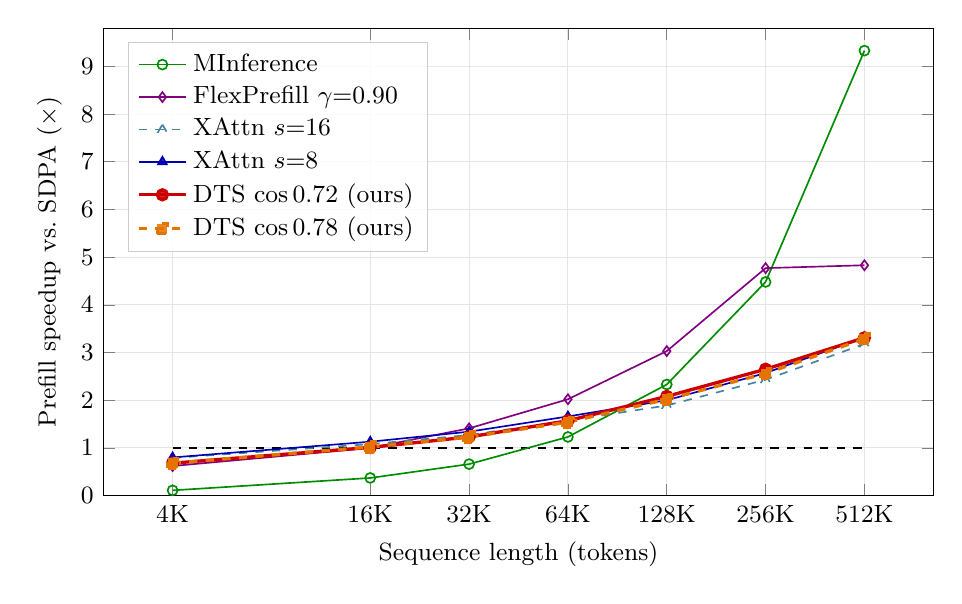
\begin{tikzpicture}
\begin{axis}[
    width=\linewidth, height=0.62\linewidth,
    xmode=log, log basis x=2,
    xtick={4096,16384,32768,65536,131072,262144,524288},
    xticklabels={4K,16K,32K,64K,128K,256K,512K},
    xlabel={Sequence length (tokens)},
    ylabel={Prefill speedup vs.\ SDPA ($\times$)},
    ymin=0, ymax=9.8,
    ytick={0,1,2,3,4,5,6,7,8,9},
    grid=both, grid style={gray!20},
    legend pos=north west,
    legend cell align=left,
    legend style={font=\small, fill=white, fill opacity=0.85, text opacity=1, draw=gray!40},
    tick label style={font=\small},
    label style={font=\small},
    mark size=1.8pt,
]
% break-even reference (SDPA)
\addplot[black, dashed, thick, forget plot] coordinates {(4096,1)(524288,1)};

\addplot[color=green!55!black, semithick, mark=o]
    coordinates {(4096,0.11)(16384,0.37)(32768,0.66)(65536,1.23)(131072,2.33)(262144,4.48)(524288,9.33)};
\addlegendentry{MInference}
\addplot[color=violet, semithick, mark=diamond]
    coordinates {(4096,0.62)(16384,1.00)(32768,1.41)(65536,2.02)(131072,3.03)(262144,4.77)(524288,4.83)};
\addlegendentry{FlexPrefill $\gamma{=}0.90$}
\addplot[color=cyan!60!black, semithick, dashed, mark=triangle]
    coordinates {(4096,0.79)(16384,1.08)(32768,1.27)(65536,1.57)(131072,1.89)(262144,2.43)(524288,3.18)};
\addlegendentry{XAttn $s{=}16$}
\addplot[color=blue!70!black, semithick, mark=triangle*]
    coordinates {(4096,0.80)(16384,1.13)(32768,1.34)(65536,1.66)(131072,2.00)(262144,2.57)(524288,3.32)};
\addlegendentry{XAttn $s{=}8$}
\addplot[color=red!80!black, very thick, mark=*]
    coordinates {(4096,0.68)(16384,1.01)(32768,1.23)(65536,1.57)(131072,2.08)(262144,2.65)(524288,3.31)};
\addlegendentry{DTS cos\,0.72 (ours)}
\addplot[color=orange!90!black, very thick, dashed, mark=square*]
    coordinates {(4096,0.68)(16384,1.02)(32768,1.23)(65536,1.54)(131072,2.02)(262144,2.56)(524288,3.29)};
\addlegendentry{DTS cos\,0.78 (ours)}
\end{axis}
\end{tikzpicture}
\caption{End-to-end prefill speedup relative to SDPA across sequence lengths on LLaMA-3.1 8B Instruct (4$\times$H100, layer-sharded). Points above the dashed break-even line (1.0$\times$) are faster than full attention.}
\label{fig:dts_speedup_trend}
\end{figure}

\subsection{Cosine threshold ablation}
\label{sec:results_cos_ablation}

The cosine threshold $\tau$ controls how aggressively DTS packs the delta representation used for tile scoring: a lower $\tau$ keeps fewer rows, making the score cheaper but less accurate, while a higher $\tau$ keeps more rows for a more accurate but more expensive score. We sweep $\tau \in \{0.70, 0.72, 0.75, 0.78, 0.80\}$ at fixed recall $r{=}0.90$ and report speedup, RULER, and LongBench. Because this sweep repeats the evaluation across five configurations, we use the reduced RULER (30 samples, 9 tasks) and reduced LongBench (9 tasks).

The sweep trades scoring cost against tile count, and the two roughly cancel out (Table~\ref{tab:cos_ablation}). Lower thresholds score faster (1.6\% of full tile cost, 1{,}447 ms at cos\,0.70) but need more tiles to reach 90\% attention mass, since the ranking is coarser (19.0\% of tiles, 3{,}094 ms of attention). Higher thresholds give a sharper ranking that hits the same recall with fewer tiles (13.3\% of tiles, 2{,}140 ms of attention at cos\,0.80) but cost more to score (8.7\%, 2{,}885 ms). Because scoring and attention move in opposite directions, the end-to-end speedup stays roughly flat: it peaks at cos\,0.72 (2.10$\times$), stays close at cos\,0.70 (2.08$\times$), and only drops off at the high end (2.03$\times$ at cos\,0.78, 1.97$\times$ at cos\,0.80).

RULER is essentially lossless across the whole sweep (Table~\ref{tab:cos_ablation}): every setting lands within 0.4 points of the others.

LongBench is more sensitive to $\tau$ (Table~\ref{tab:cos_ablation}). Accuracy peaks at cos\,0.72 (39.21) and falls off at both ends. cos\,0.72 is the best overall choice: fastest and best on LongBench. cos\,0.78 is the accuracy-maximizing choice, holding the best RULER score (91.80) at a still-good 2.03$\times$. We carry both forward as the two settings compared against the other methods.

\begin{table}[!ht]
\centering
\caption{End-to-end prefill speedup (128K tokens) and accuracy (\%) on RULER and LongBench for DTS cosine thresholds on LLaMA-3.1 8B Instruct. Attention density is the fraction of computed sparse attention. Score\% represents the scoring overhead. Score ms and Attn ms indicate the respective phase latencies.}
\label{tab:cos_ablation}
\resizebox{\linewidth}{!}{%
\begin{tabular}{lrrrrrrr}
\toprule
Method & Speedup & Density & Score\% & Score (ms) & Attn (ms) & RULER & LongBench \\
\midrule
Full attention & 1.00$\times$ & 100\% & -- & -- & -- & 91.52 & 39.54 \\
\midrule
cos\,0.70 & 2.08$\times$ & 19.0\% & 1.6\% & 1{,}447 & 3{,}094 & 91.69 & 38.95 \\
cos\,0.72 & 2.10$\times$ & 17.6\% & 2.3\% & 1{,}611 & 2{,}853 & 91.51 & 39.21 \\
cos\,0.75 & 2.09$\times$ & 15.7\% & 3.8\% & 1{,}954 & 2{,}545 & 91.42 & 39.08 \\
cos\,0.78 & 2.03$\times$ & 14.2\% & 6.3\% & 2{,}445 & 2{,}284 & 91.80 & 39.15 \\
cos\,0.80 & 1.97$\times$ & 13.3\% & 8.7\% & 2{,}885 & 2{,}140 & 91.58 & 38.61 \\
\bottomrule
\end{tabular}%
}
\end{table}
\subsection{Cross-Model Generalization: Qwen2.5-7B}
\label{sec:results_qwen}

The results above use LLaMA-3.1 8B Instruct throughout. To check whether DTS's behavior is specific to that model, we repeat the full RULER, LongBench, and speedup evaluation on Qwen2.5-7B-Instruct-1M, using the same two operating points (cos\,0.72 and cos\,0.78) and the same baselines.


\paragraph{RULER.}

Table~\ref{tab:delta_tile_scoring_qwen} reports RULER accuracy on Qwen. MInference (90.35) and both XAttention strides (90.25 at $s{=}16$, 90.23 at $s{=}8$) tie full attention (90.33); DTS trails by 1.4--2.2 points (88.89 at cos\,0.78 and 88.12 at cos\,0.72). FlexPrefill collapses to 53.50.

\begin{table}[!ht]
\centering
\caption{RULER accuracy (\%) comparing DTS with the other baselines on Qwen2.5-7B-Instruct-1M. Best score per column in \textbf{bold}. The DTS row is measured under the corrected scoring kernel; cos\,0.72 was not re-run under it and is omitted.}
\label{tab:delta_tile_scoring_qwen}
\resizebox{\linewidth}{!}{%
\begin{tabular}{lrrrrrrr}
\toprule
Method & 4K & 8K & 16K & 32K & 64K & 128K & Avg \\
\midrule
Full attention              & 94.10 & 93.67 & 93.54 & \textbf{91.17} & 88.07 & \textbf{81.41} & 90.33 \\
MInference                  & \textbf{94.16} & \textbf{94.00} & \textbf{94.03} & 90.99 & 87.68 & 81.23 & \textbf{90.35} \\
FlexPrefill                  & 74.39 & 61.74 & 55.66 & 59.71 & 32.38 & 37.10 & 53.50 \\
\midrule
XAttn $s{=}16$                & 94.02 & 93.55 & 93.66 & 90.85 & \textbf{88.21} & 81.22 & 90.25 \\
XAttn $s{=}8$                 & 94.06 & 93.53 & 93.60 & 91.02 & 87.96 & 81.23 & 90.23 \\
\midrule
DTS cos\,0.78 & 93.98 & 93.49 & 93.33 & 89.47 & 86.95 & 81.28 & 89.75 \\
\bottomrule
\end{tabular}%
}
\end{table}

To trace the source of this performance gap, we analyze the 13 individual RULER tasks at 128K. While DTS matches or beats XAttention on 11 tasks, it falls short on variable tracking (vt) and common word extraction (cwe). Both are aggregation tasks that require combining information from multiple positions rather than retrieving a single needle. DTS's performance drops sharply on these (e.g., 53.8 and 13.8 at cos\,0.72, compared to full attention's 75.8 and 27.3), indicating a trade-off where DTS remains strong on retrieval but struggles with broad aggregation.

\paragraph{LongBench.}

Table~\ref{tab:longbench_qwen} shows LongBench scores on Qwen. DTS ties full attention (46.76): 46.19 at cos\,0.72 and 46.20 at cos\,0.78, tracking both XAttention variants (46.46 at $s{=}8$, 46.66 at $s{=}16$).

DTS only underperforms full attention on MuSiQue (29.22--29.88 vs. 32.70) and 2WikiMultiHopQA (52.46--53.31 vs. 55.45). Because both are multi-hop tasks that require synthesizing evidence across passages, this result reinforces the aggregation limitation observed in RULER. Additionally, MInference's average is marked with a $\dagger$ because it failed to complete QMSum and RepoBench-P at 128K.

\begin{table*}[!ht]
\centering
\small
\caption{LongBench scores on Qwen2.5-7B-Instruct-1M. Task abbreviations as in Table~\ref{tab:longbench}. Best score per column in \textbf{bold}. As in Table~\ref{tab:delta_tile_scoring_qwen}, the DTS row is measured under the corrected scoring kernel; cos\,0.72 was not re-run under it and is omitted. $\dagger$MInference failed on 2 of 16 tasks (QMSum, RepoBench-P); no average is reported for it, since a mean over the 14 completed tasks omits two below-average tasks and is not comparable to the other rows.}
\label{tab:longbench_qwen}
\resizebox{\linewidth}{!}{%
\begin{tabular}{lrrrrrrrrrrrrrrrrr}
\toprule
Method & NQA & Qas & MFQ & HotP & 2Wiki & Mus & GovR & QMS & MNews & TREC & TQA & SAM & PCnt & PassR & LCC & RepoB & Avg \\
\midrule
Full attention               & 29.26 & 45.12 & 51.49 & \textbf{58.34} & 55.45 & 32.70 & 35.22 & 23.99 & 25.69 & 71.00 & 83.31 & 45.24 & 10.00 & \textbf{100.00} & 48.40 & 32.92 & 46.76 \\
MInference$^\dagger$         & 29.38 & 45.36 & 51.85 & 56.77 & 54.65 & \textbf{33.47} & 35.20 & --    & 25.98 & 71.00 & 83.31 & \textbf{46.32} & 10.00 & 99.00 & 47.63 & --    & --    \\
FlexPrefill                  & 24.68 & 39.46 & 50.63 & 48.72 & 50.58 & 21.06 & 33.61 & \textbf{24.67} & 25.42 & 70.00 & 78.64 & 46.11 & 2.00 & 59.00 & 45.18 & 33.61 & 40.84 \\
XAttn $s{=}16$               & 29.84 & 44.74 & 51.41 & 57.63 & \textbf{55.62} & 32.60 & 34.84 & 24.00 & \textbf{26.09} & 70.00 & 83.18 & 46.00 & \textbf{12.00} & \textbf{100.00} & 46.70 & 31.97 & 46.66 \\
XAttn $s{=}8$                & \textbf{30.26} & \textbf{45.77} & 52.31 & 58.16 & 53.78 & 31.62 & 35.18 & 24.09 & 26.00 & 71.00 & 83.51 & 45.83 & 9.00 & \textbf{100.00} & 45.14 & 31.70 & 46.46 \\
\midrule
DTS cos\,0.78 & 21.96 & 44.66 & \textbf{53.08} & 54.57 & 54.63 & 33.21 & \textbf{35.47} & 24.12 & 25.64 & \textbf{74.00} & \textbf{84.19} & 46.13 & 6.00 & \textbf{100.00} & \textbf{48.49} & \textbf{33.71} & 46.24 \\
\bottomrule
\end{tabular}%
}
\end{table*}

\paragraph{Speedup.}

Figure~\ref{fig:dts_speedup_trend_qwen} illustrates end-to-end speedups on Qwen up to 512K (DTS and XAttention are capped at 256K due to OOM errors). The trends largely reflect those seen on LLaMA. MInference is the slowest up to 64K but overtakes FlexPrefill at 512K, reaching 4.81$\times$ (a smaller gain than on LLaMA). FlexPrefill is the fastest up to 256K before dipping to 3.87$\times$ at 512K. DTS and XAttention perform similarly, though DTS maintains a clear speed advantage at 128K and 256K (1.57$\times$ and 1.81$\times$ vs. XAttention's 1.45$\times$ and 1.74$\times$).

\begin{figure}[!ht]
\centering
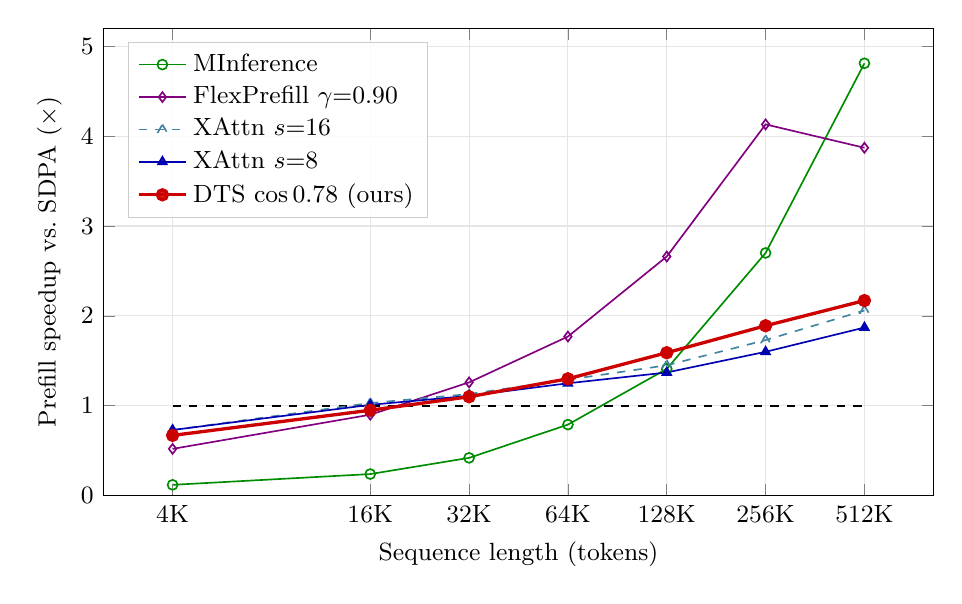
\begin{tikzpicture}
\begin{axis}[
    width=\linewidth, height=0.62\linewidth,
    xmode=log, log basis x=2,
    xtick={4096,16384,32768,65536,131072,262144,524288},
    xticklabels={4K,16K,32K,64K,128K,256K,512K},
    xlabel={Sequence length (tokens)},
    ylabel={Prefill speedup vs.\ SDPA ($\times$)},
    ymin=0, ymax=5.2,
    ytick={0,1,2,3,4,5},
    grid=both, grid style={gray!20},
    legend pos=north west,
    legend cell align=left,
    legend style={font=\small, fill=white, fill opacity=0.85, text opacity=1, draw=gray!40},
    tick label style={font=\small},
    label style={font=\small},
    mark size=1.8pt,
]
% break-even reference (SDPA)
\addplot[black, dashed, thick, forget plot] coordinates {(4096,1)(524288,1)};

\addplot[color=green!55!black, semithick, mark=o]
    coordinates {(4096,0.12)(16384,0.24)(32768,0.42)(65536,0.79)(131072,1.41)(262144,2.70)(524288,4.81)};
\addlegendentry{MInference}
\addplot[color=violet, semithick, mark=diamond]
    coordinates {(4096,0.52)(16384,0.90)(32768,1.26)(65536,1.77)(131072,2.66)(262144,4.13)(524288,3.87)};
\addlegendentry{FlexPrefill $\gamma{=}0.90$}
\addplot[color=cyan!60!black, semithick, dashed, mark=triangle]
    coordinates {(4096,0.73)(16384,1.03)(32768,1.13)(65536,1.29)(131072,1.45)(262144,1.73)(524288,2.06)};
\addlegendentry{XAttn $s{=}16$}
\addplot[color=blue!70!black, semithick, mark=triangle*]
    coordinates {(4096,0.73)(16384,1.01)(32768,1.11)(65536,1.25)(131072,1.37)(262144,1.60)(524288,1.87)};
\addlegendentry{XAttn $s{=}8$}
\addplot[color=red!80!black, very thick, mark=*]
    coordinates {(4096,0.67)(16384,0.95)(32768,1.10)(65536,1.30)(131072,1.59)(262144,1.89)(524288,2.17)};
\addlegendentry{DTS cos\,0.78 (ours)}
\end{axis}
\end{tikzpicture}
\caption{End-to-end prefill speedup relative to SDPA across sequence lengths on Qwen2.5-7B-Instruct-1M (4$\times$H100, layer-sharded). Points above the dashed break-even line (1.0$\times$) are faster than full attention.}
\label{fig:dts_speedup_trend_qwen}
\end{figure}

\subsection{Video Understanding: Qwen2-VL}
\label{sec:results_video}

We evaluate DTS on Video-MME (1 fps, no subtitles) using Qwen2-VL-7B-Instruct. We empirically observed that packing by Euclidean distance yields better performance on video tokens than cosine similarity, so we report DTS using Euclidean packing (see Appendix~\ref{app:videomme_ablations} for this ablation study). We measure accuracy on the full test set (2,700 videos) and prefill speedup (attention latency only) on a 10-video timing sample per duration split. 

Table~\ref{tab:videomme_main} reports results against the same baselines used in text experiments. DTS at $\delta{=}15$ is our primary configuration. It closely tracks full attention accuracy (60.8 vs. 62.1 overall) while providing the best balance of speed and accuracy on the critical long-video split: it scores 52.6 and runs at 1.33$\times$ full attention, outperforming XAttention (51.7, 1.18$\times$). MInference retains the highest accuracy (62.4) but remains slower than full attention across all buckets. FlexPrefill provides the highest speedup (2.18$\times$) but trails DTS in long-video accuracy (51.6).

\begin{table}[!ht]
\centering
\caption{Video-MME accuracy and prefill speedup on Qwen2-VL-7B-Instruct (Video-MME @ 1fps, no subtitles). Accuracy (\%) is on the full test set ($n{=}2700$). Speedup ($\times$full) is attention-kernel latency (self\_attn\_ms) relative to full attention on a 10-videos-per-bucket timing sample. Best accuracy per column in \textbf{bold}.}
\label{tab:videomme_main}
\resizebox{\linewidth}{!}{%
\begin{tabular}{lrrrrrrr}
\toprule
 & \multicolumn{4}{c}{Accuracy (\%)} & \multicolumn{3}{c}{Speedup ($\times$full)} \\
\cmidrule(lr){2-5}\cmidrule(lr){6-8}
Method & Short & Med & Long & Avg & Short & Med & Long \\
\midrule
Full attention                    & 72.3 & 61.0 & 53.0 & 62.1 & 1.00 & 1.00 & 1.00 \\
MInference                        & \textbf{72.8} & 61.2 & \textbf{53.3} & \textbf{62.4} & 0.42 & 0.62 & 0.61 \\
FlexPrefill                        & 72.1 & \textbf{61.3} & 51.6 & 61.7 & 1.41 & 2.12 & 2.18 \\
XAttn $s{=}16$                    & 72.0 & 59.9 & 51.7 & 61.2 & 0.95 & 1.22 & 1.18 \\
\midrule
DTS $\delta{=}15$                 & 71.1 & 58.6 & 52.6 & 60.8 & 0.98 & 1.21 & 1.33 \\
\bottomrule
\end{tabular}%
}
\end{table}


\section{Conclusion}


Among the baselines we tested, there is no silver bullet. Each method trades speed against accuracy and generalization in a different way. The shape-oriented methods (MInference and FlexPrefill) excel in speedup, yet FlexPrefill struggles with model generalization and MInference realizes its speedup late.

MInference reaches exceptional speedups at very long contexts (256K to 512K), but it rises late and is slower than the baseline up to 128K on Qwen2.5. This shows up on video, where the longest clips sit around 32K tokens and MInference is much slower than full attention (0.42$\times$ to 0.62$\times$). It holds up accuracy and generalizes to models well. However, its RULER accuracy degrades at 128K on LLaMA (63.73 versus 74.46 for full attention). Overall, its solid performance proves its place in production.

FlexPrefill has a smoother speedup curve. It delivers speedups at shorter contexts even though it cannot reach the dramatic 512K speedup of MInference. Although it is competitive on speed, it suffers accuracy degradation on LLaMA RULER's 128K (74.23 versus 74.46) and on LongBench average (44.78 versus 47.53). More importantly, its accuracy breaks on every Qwen text benchmark (RULER 53.50 versus 90.33), which points to a cross-model generalization failure.

The block-sparse methods (XAttention and DTS) retain accuracy better across the benchmarks, yet they cannot reach the impressive speedups of the shape-oriented methods.

XAttention generally has solid accuracy retention and cleanly generalizes to different models and modalities. On the Qwen RULER benchmark it scores considerably higher than DTS (90.25 versus 88.12--88.89), but it falls back on LLaMA compared to DTS (88.02 versus 89.02 on RULER). Its overall accuracy is tied with DTS on video, yet on the long bucket DTS has an advantage (52.6 versus 51.7) while providing higher speedup (1.33$\times$ versus 1.18$\times$).


Overall DTS generally excels at accuracy retention and shows solid model and modality generalization. The one exception is the Qwen RULER aggregation tasks (variable tracking and common word extraction), where its accuracy degrades, though this does not carry over to the real-world LongBench benchmark. It is the best method for accuracy retention on LLaMA and in long video understanding. Compared to XAttention, at all configurations and sequence lengths, it either matches or beats XAttention's speedup due to its much lighter scoring phase. The only reason we cannot say it dominates XAttention is the Qwen RULER aggregation degradation.


\subsection{Future Work}

Several directions could push DTS further. First, thresholding can be refined by applying separate limits to $Q$ and $K$, or using more aggressive thresholds in later layers. Second, DTS currently lacks a tile normalization scheme, meaning that some tiles inherently score higher simply because they contain more unpruned vectors. Finally, future work will evaluate DTS on larger models, test it on the InfiniBench benchmark, and apply it to image and video generation tasks.

\newpage
\bibliographystyle{IEEEtran}
\bibliography{references}

\appendices
\section{Per-Head $\tau$ Calibration Details}
\label{app:calibration}

To achieve the exact target retention of attention mass despite the tile scores being only estimates, we employ an offline calibration procedure for the threshold $\tau$. Specifically, we process a calibration set through the network and compute both the estimated tile scores from $\hat{\textbf{Q}}$ and $\hat{\textbf{K}}$ as well as the exact attention mass. For each head, we adjust its threshold $\tau_h$ until the actual retained attention mass matches the desired target (e.g., $90\%$). These per-head thresholds are then fixed and used during inference, ensuring reliable and uniform sparsity scaling across layers.
\section{Video-MME Ablations}
\label{app:videomme_ablations}

Table~\ref{tab:videomme_ablation_metric} sweeps packing metrics on a 200-video subset. Euclidean distance consistently outperforms cosine similarity on long videos. Our chosen operating point, $\delta{=}15$, achieves the highest overall (60.5) and long-video (50.0) scores. While its scoring ratio (9.7\%) is higher than XAttention's (6.25\%), it retains significantly fewer tiles (30.5\% vs. 40.7\%), making it faster end-to-end. A more aggressive threshold, $\delta{=}19$, drops the scoring ratio to 1.4\% and retains only 23.6\% of tiles, offering a promising high-speed alternative at the cost of some accuracy.

\begin{table}[!ht]
\centering
\caption{Packing metric ablation on Video-MME (200-video subset), Qwen2-VL-7B-Instruct, recall $r{=}0.90$, count-weighting off throughout.}
\label{tab:videomme_ablation_metric}
\resizebox{\linewidth}{!}{%
\begin{tabular}{llrrrrrr}
\toprule
Metric & $\tau$/$\delta$ & Overall & Short & Medium & Long & Retained tiles & Scoring ratio \\
\midrule
XAttn $s{=}16$ & -- & 59.0 & 75.0 & 59.7 & 44.6 & 40.7\% & 6.25\% \\
\midrule
Cosine & $\tau{=}0.90$ & 59.5 & 78.1 & 54.8 & 47.3 & 33.6\% & 45.8\% \\
Cosine & $\tau{=}0.80$ & 58.5 & 76.6 & 56.5 & 44.6 & 32.4\% & 14.2\% \\
Cosine & $\tau{=}0.75$ & 56.5 & 79.7 & 48.4 & 43.2 & 30.6\% & 7.4\% \\
Cosine & $\tau{=}0.72$ & 58.5 & 81.2 & 50.0 & 45.9 & 29.3\% & 5.0\% \\
\midrule
Euclidean & $\delta{=}13$ & 59.5 & 78.1 & 56.5 & 45.9 & 32.8\% & 21.2\% \\
Euclidean & $\delta{=}15$ & 60.5 & 76.6 & 56.5 & 50.0 & 30.5\% & 9.7\% \\
Euclidean & $\delta{=}17$ & 58.5 & 76.6 & 53.2 & 47.3 & 27.1\% & 3.8\% \\
Euclidean & $\delta{=}19$ & 57.5 & 75.0 & 48.4 & 50.0 & 23.6\% & 1.4\% \\
\bottomrule
\end{tabular}%
}
\end{table}

\end{document}
